% Provenance (never printed): cycle 2 "Questionner le monde" (states of water in
% weather phenomena; daily observation), see sources/book1/PROVENANCE.md.
% Book 1, grade 1, chapter 1. No real-world number in this chapter.
\chapter{Observando o tempo}\label{ch:g1:watching-the-weather}

É bem cedinho. Lena acorda, sobe na cadeira perto da janela do quarto
e olha lá para fora. O céu está cinzento. Gotinhas de água escorrem
pelo vidro. Os telhados do outro lado da rua estão molhados e
brilhantes, e a árvore do quintal está pingando.

``Que roupa eu vou usar hoje?'', ela pergunta.

Para responder, Lena não precisa de livro nem de máquina. Basta olhar
pela janela. A janela é a sua primeira estação meteorológica.

\begin{omfigure}
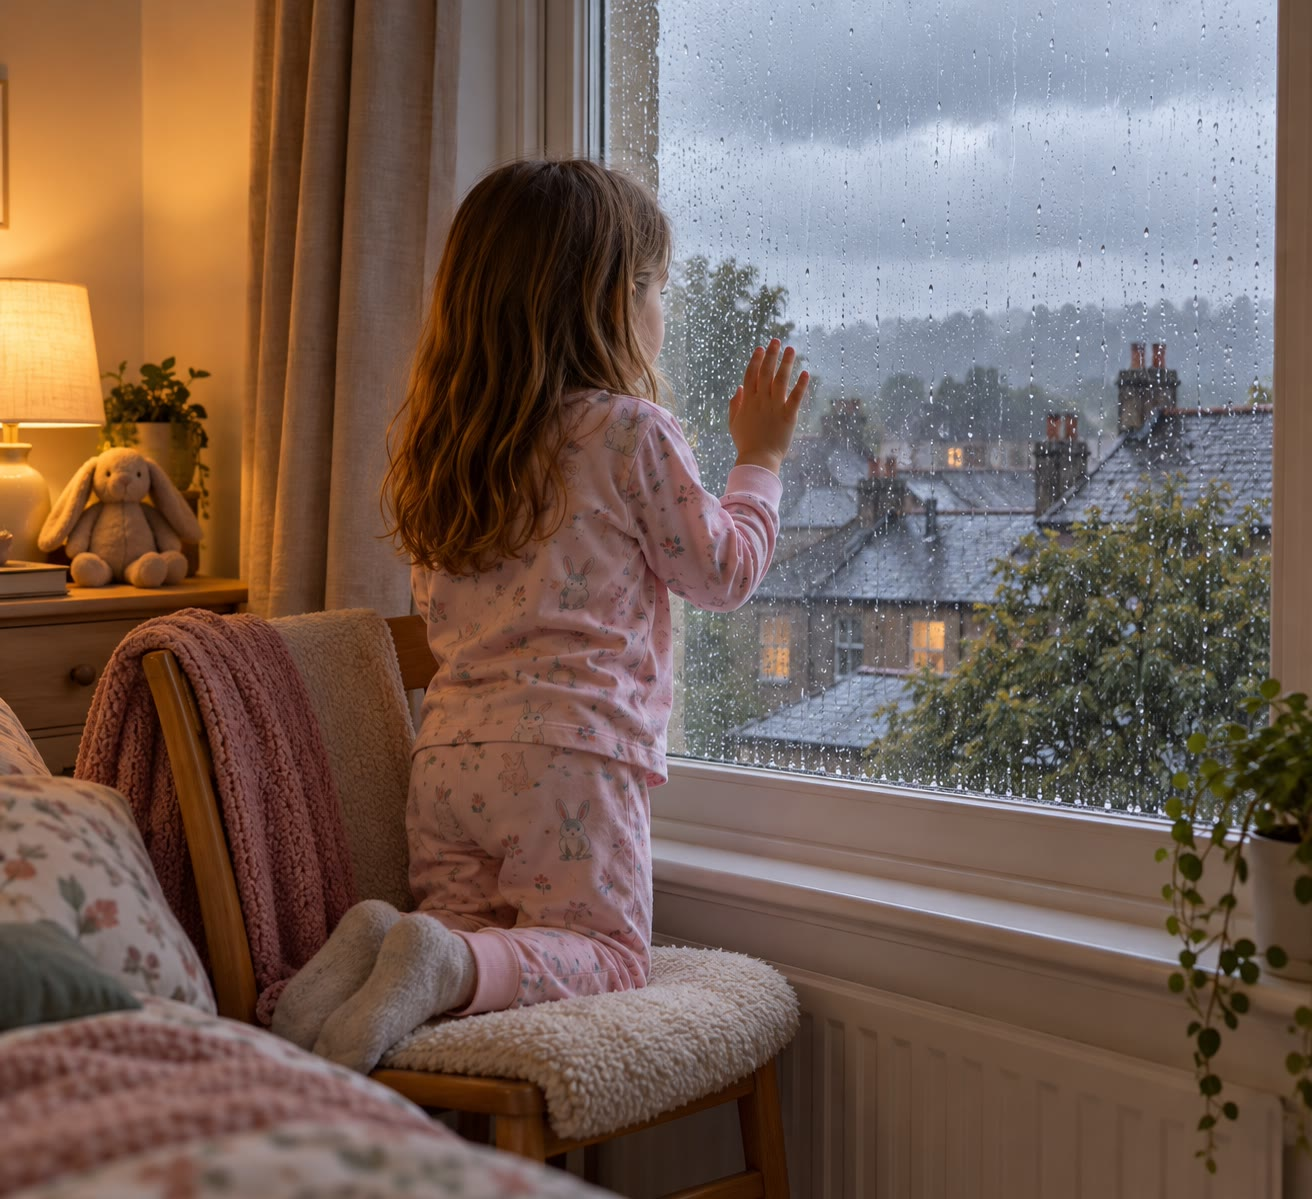
\includegraphics[width=0.72\linewidth]{images/book1/ai/g1-rainy-window.jpg}

{\small Uma manhã cinzenta e chuvosa vista pela janela.}
\end{omfigure}

\begin{recall}
Toda manhã o Sol nasce e o dia começa; toda tarde ele se põe e a noite
chega. Nos livros de física você viu por que a noite vem depois do dia.
Neste capítulo vamos olhar para outra coisa que muda sem parar: o
\omterm{def:g1:watching-the-weather:weather}{tempo} que faz lá fora.
\end{recall}

\section{O que é o tempo?}

Quando saímos de casa, sentimos o ar no rosto. Ele pode estar quente ou
frio. Pode estar parado, ou pode empurrar o nosso cabelo e a nossa roupa:
então está ventando. Olhamos para o céu. Ele pode estar azul e claro, ou
coberto de nuvens. Às vezes cai chuva das nuvens, às vezes neve. Tudo isso
junto é o \omterm{def:g1:watching-the-weather:weather}{tempo}.

\begin{definition}[Tempo]\label{def:g1:watching-the-weather:weather}
O \emph{tempo}\index{tempo} é como estão o ar e o céu num lugar, num
certo momento: ensolarado ou nublado, seco, chuvoso ou com neve, calmo ou
com vento, quente ou frio.
\end{definition}

Para descrever o \omterm{def:g1:watching-the-weather:weather}{tempo}, respondemos a algumas perguntas simples:
\begin{enumerate}
  \item \textbf{Como está o céu?} Está azul, com o Sol brilhando? Há
        algumas nuvens, ou o céu está todo cinzento?
  \item \textbf{Está caindo alguma coisa do céu?} Chuva? Neve? Nada?
  \item \textbf{Está ventando?} As folhas das árvores se mexem? Uma
        bandeira tremula?
  \item \textbf{Está quente ou frio?} Precisamos de casaco?
\end{enumerate}

\begin{omfigure}
\begin{minipage}[b]{0.49\linewidth}\centering
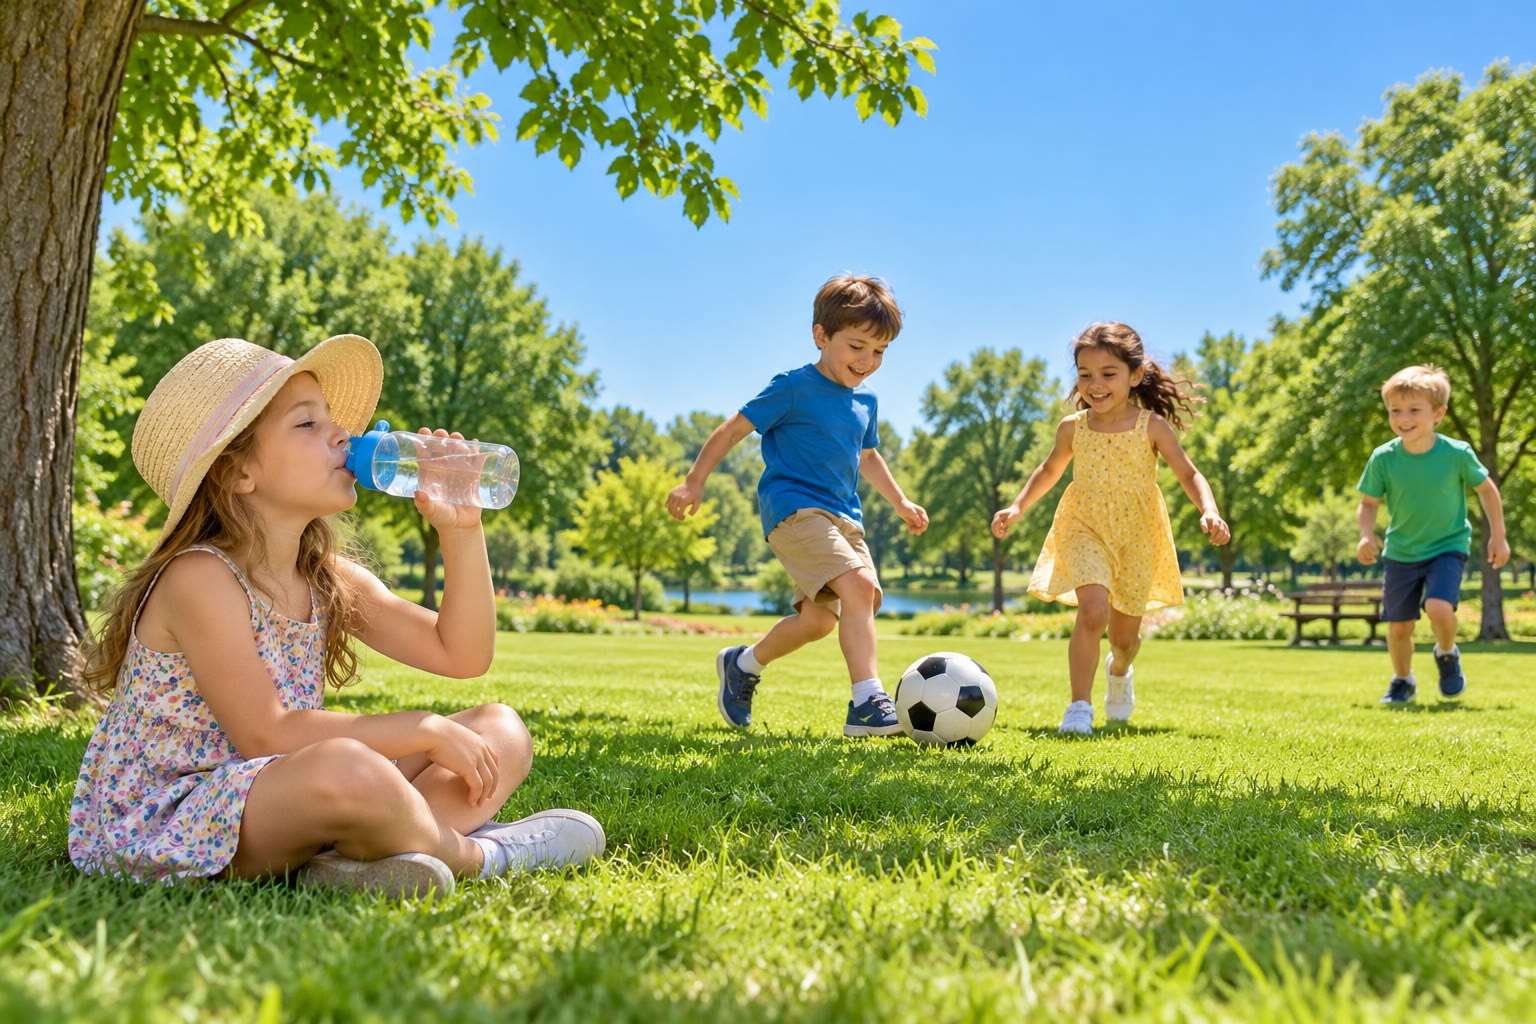
\includegraphics[width=\linewidth]{images/book1/ai/g1-sunny-park.jpg}

{\small Ensolarado e quente.}
\end{minipage}\hfill
\begin{minipage}[b]{0.49\linewidth}\centering
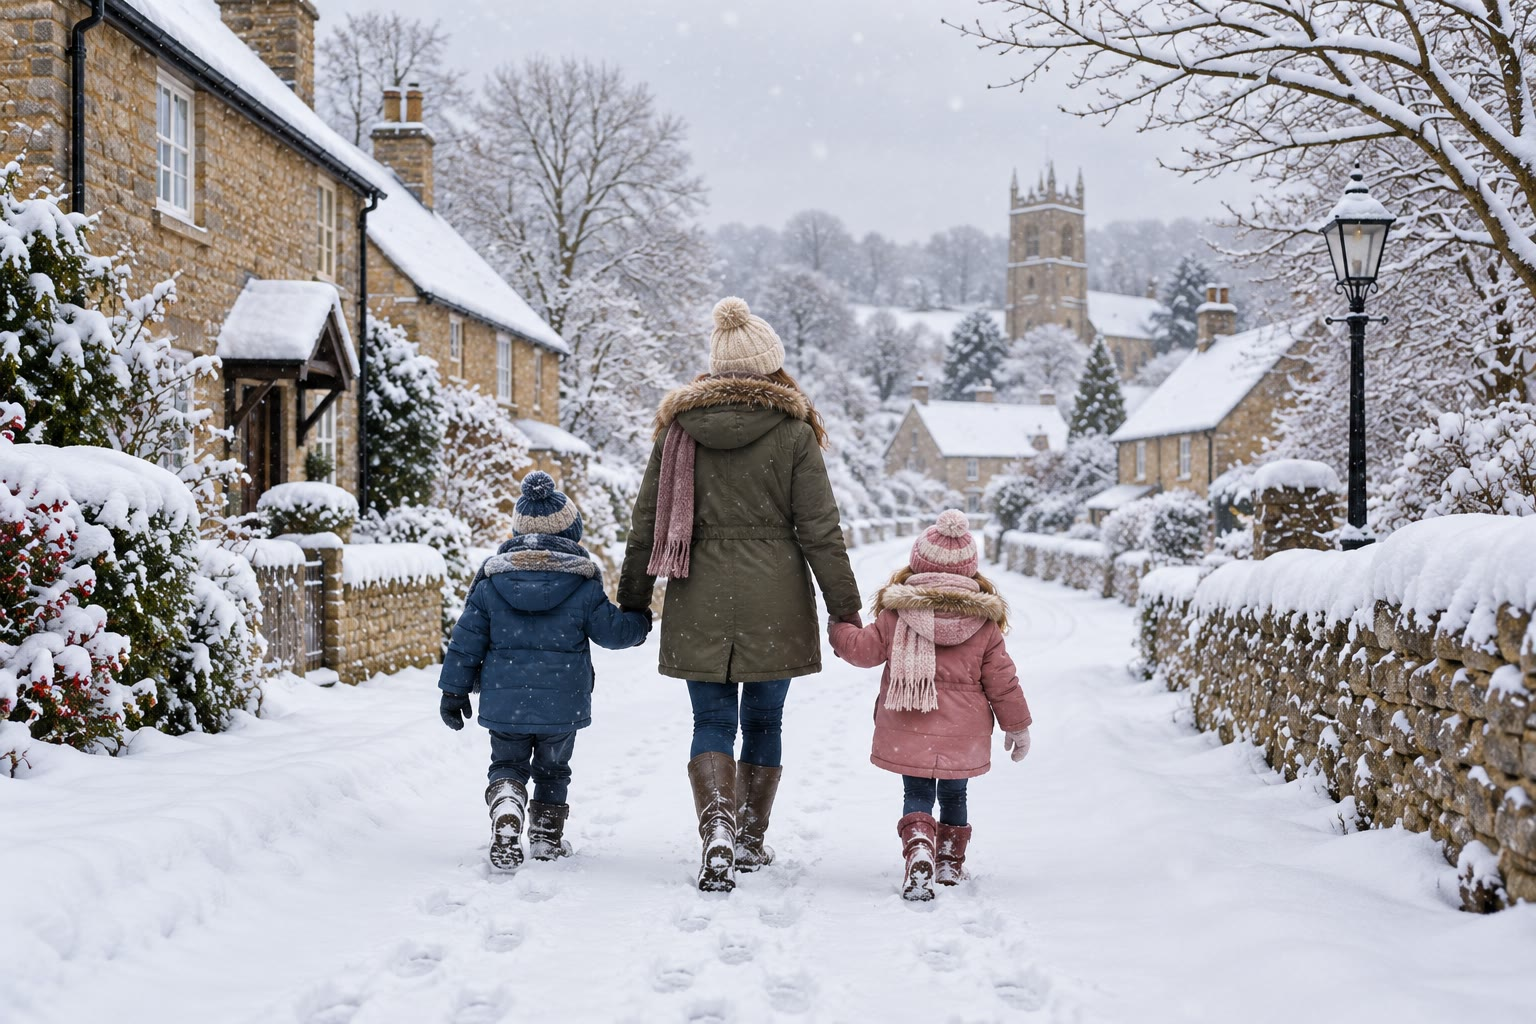
\includegraphics[width=\linewidth]{images/book1/ai/g1-snowy-street.jpg}

{\small Com neve e frio.}
\end{minipage}

\medskip
\begin{minipage}[b]{0.49\linewidth}\centering
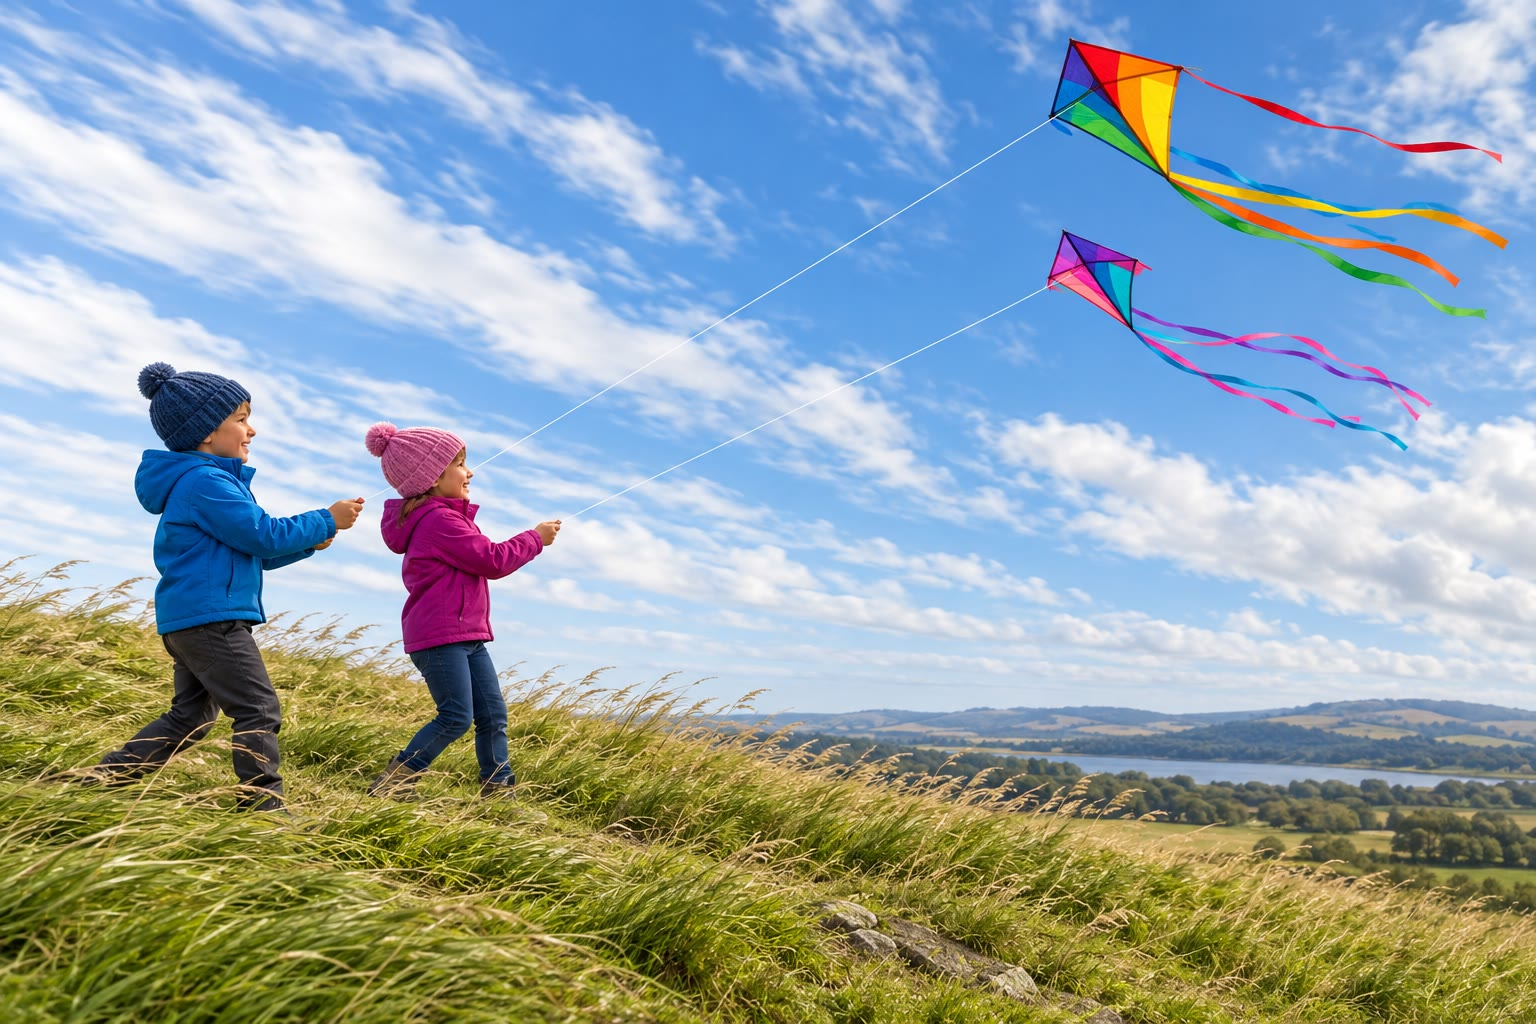
\includegraphics[width=\linewidth]{images/book1/ai/g1-windy-kites.jpg}

{\small Com vento: as pipas voam.}
\end{minipage}\hfill
\begin{minipage}[b]{0.49\linewidth}\centering
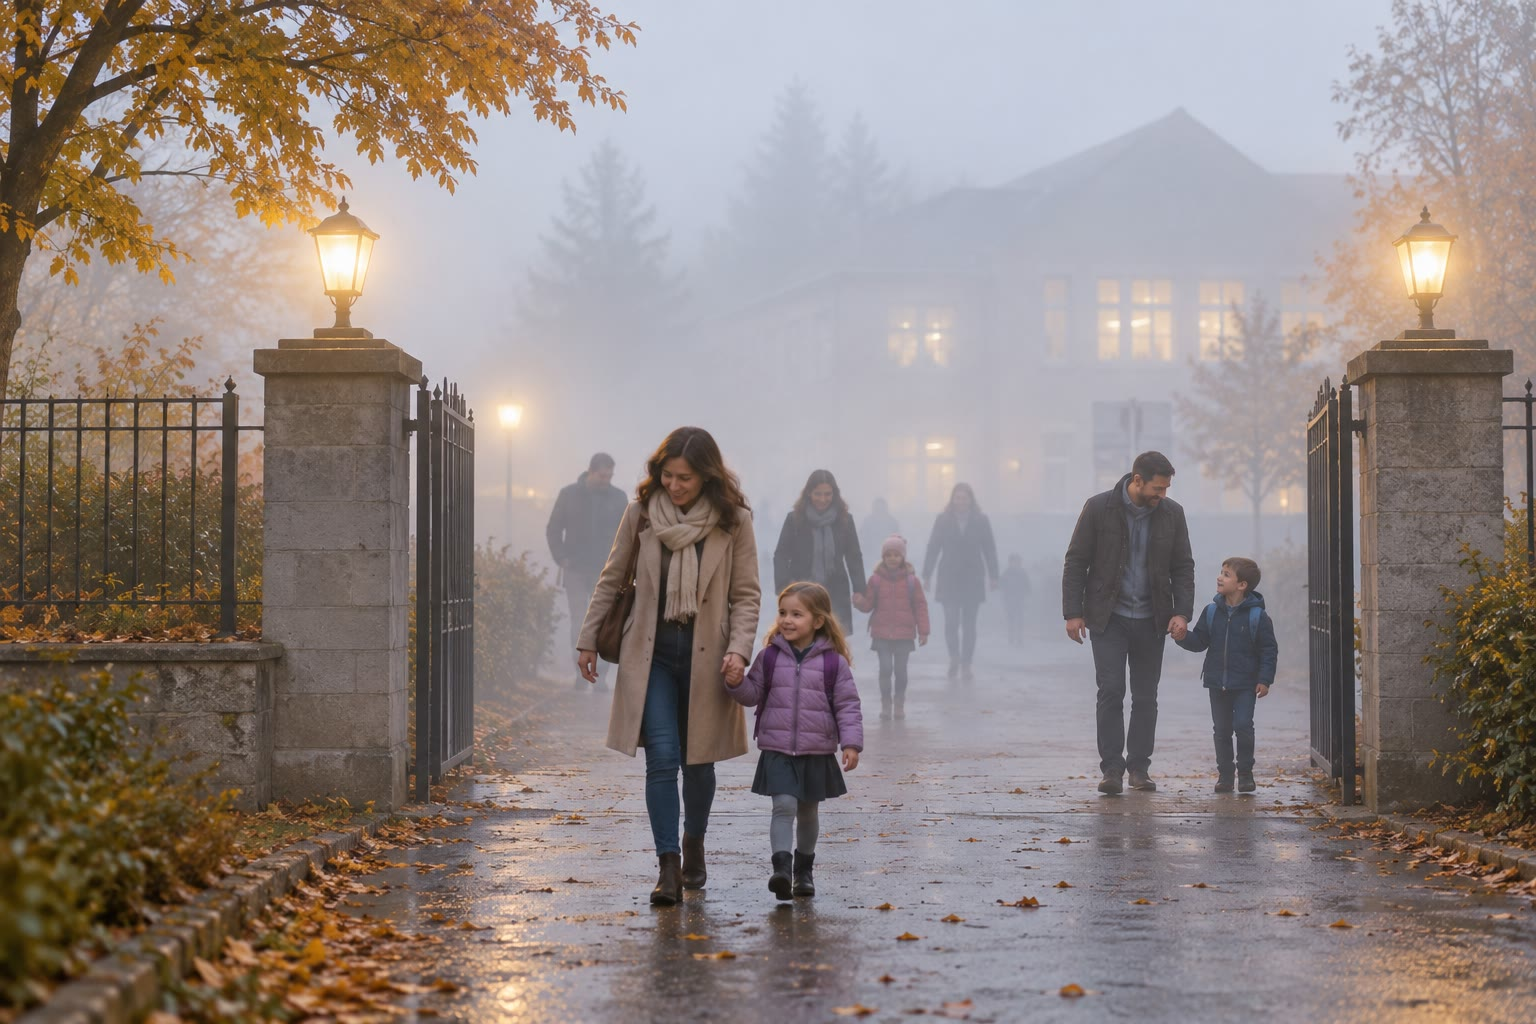
\includegraphics[width=\linewidth]{images/book1/ai/g1-foggy-school.jpg}

{\small Com neblina: não dá para ver longe.}
\end{minipage}
\end{omfigure}

\begin{example}[Neblina]\label{ex:g1:watching-the-weather:fog}
Em algumas manhãs o próprio ar parece branco, e as árvores no fim da rua
parecem sumir. É a neblina. A neblina é uma nuvem que encosta no chão.
Quando o dia esquenta, a neblina muitas vezes vai embora.
\end{example}

\section{Os símbolos do tempo e o quadro do tempo}

Descrever o \omterm{def:g1:watching-the-weather:weather}{tempo} com palavras demora muito. Quem observa o \omterm{def:g1:watching-the-weather:weather}{tempo} usa, em
vez disso, desenhos pequenos: os \omterm{def:g1:watching-the-weather:weather-chart}{símbolos do tempo}. Cada símbolo é fácil
de desenhar e fácil de reconhecer.

\begin{omfigure}
\begin{tikzpicture}[x=1cm, y=1cm]
  \foreach \i/\n/\t in {0/sun/ensolarado, 1/suncloud/sol e nuvens,
      2/cloud/nublado, 3/rain/chuvoso, 4/shower/pancadas de chuva} {
    \pic[scale=1.25, transform shape] at (\i*2.6,0) {omwx=\n};
    \node[font=\small, align=center, text width=2.4cm] at (\i*2.6,-1.05) {\t};
  }
  \foreach \i/\n/\t in {0/snow/com neve, 1/storm/trovoada, 2/fog/com neblina,
      3/wind/com vento} {
    \pic[scale=1.25, transform shape] at (\i*2.6+1.3,-2.6) {omwx=\n};
    \node[font=\small, align=center, text width=2.4cm] at (\i*2.6+1.3,-3.65) {\t};
  }
\end{tikzpicture}

{\small Nove \omterm{def:g1:watching-the-weather:weather-chart}{símbolos do tempo}. A trovoada tem uma nuvem escura e um raio;
as pancadas de chuva vêm com intervalos de sol entre elas.}
\end{omfigure}

\begin{definition}[Quadro do tempo]\label{def:g1:watching-the-weather:weather-chart}
Um \emph{símbolo do tempo}\index{simbolo do tempo@símbolo do tempo} é um desenho pequeno que mostra
um tipo de \omterm{def:g1:watching-the-weather:weather}{tempo}. Um \emph{quadro do tempo}\index{quadro do tempo} é uma tabela
em que anotamos, dia após dia, o \omterm{def:g1:watching-the-weather:weather}{tempo} que observamos, com os
símbolos do \omterm{def:g1:watching-the-weather:weather}{tempo}.
\end{definition}

Uma turma pode manter um \omterm{def:g1:watching-the-weather:weather-chart}{quadro do tempo} durante uma semana inteira. Toda
manhã, e de novo toda tarde, uma criança olha lá para fora e desenha o
símbolo no quadradinho certo. Também anotamos se está quente ou frio.

\begin{omfigure}
\begin{tikzpicture}[x=1cm, y=1cm]
  \def\cw{1.9}
  \foreach \d [count=\i from 0] in {Segunda, Terça, Quarta, Quinta,
      Sexta, Sábado, Domingo}
    \node[font=\scriptsize\bfseries] at ({1.6+\i*\cw+\cw/2},0.35) {\d};
  \node[font=\scriptsize\bfseries, anchor=east] at (1.45,-0.5) {manhã};
  \node[font=\scriptsize\bfseries, anchor=east] at (1.45,-1.5) {tarde};
  \node[font=\scriptsize\bfseries, anchor=east, align=right] at (1.45,-2.35) {quente ou\\frio?};
  \draw[black!60] (1.6,0) rectangle ({1.6+7*\cw},-2.7);
  \foreach \i in {1,...,6}
    \draw[black!60] ({1.6+\i*\cw},0.65) -- ({1.6+\i*\cw},-2.7);
  \draw[black!60] (1.6,0.65) -- ({1.6+7*\cw},0.65);
  \draw[black!60] (1.6,0.65) -- (1.6,0);
  \draw[black!60] ({1.6+7*\cw},0.65) -- ({1.6+7*\cw},0);
  \draw[black!60] (1.6,-1) -- ({1.6+7*\cw},-1);
  \draw[black!60] (1.6,-2) -- ({1.6+7*\cw},-2);
  \foreach \i/\m/\a/\w in {0/rain/rain/frio, 1/cloud/suncloud/frio,
      2/sun/sun/quente, 3/sun/suncloud/quente, 4/suncloud/shower/quente,
      5/fog/sun/quente, 6/cloud/rain/frio} {
    \pic[scale=0.8, transform shape] at ({1.6+\i*\cw+\cw/2},-0.5) {omwx=\m};
    \pic[scale=0.8, transform shape] at ({1.6+\i*\cw+\cw/2},-1.5) {omwx=\a};
    \node[font=\scriptsize] at ({1.6+\i*\cw+\cw/2},-2.35) {\w};
  }
\end{tikzpicture}

{\small O \omterm{def:g1:watching-the-weather:weather-chart}{quadro do tempo} feito por uma turma durante uma semana de primavera.}
\label{fig:g1:watching-the-weather:chart}
\end{omfigure}

\begin{method}[Ler um quadro do tempo]\label{met:g1:watching-the-weather:read}
Para ler um \omterm{def:g1:watching-the-weather:weather-chart}{quadro do tempo}:
\begin{enumerate}
  \item procure a coluna do dia que você quer;
  \item olhe a linha: manhã ou tarde;
  \item diga o \omterm{def:g1:watching-the-weather:weather}{tempo} que o símbolo mostra.
\end{enumerate}
Para saber quantos dias foram ensolarados, passe o dedo ao longo de uma
linha e conte os símbolos de sol.
\end{method}

\begin{example}[Lendo o quadro da turma]\label{ex:g1:watching-the-weather:read}
No quadro desta turma, a manhã de segunda-feira foi chuvosa e fria. Na
quarta-feira fez sol o dia todo. No sábado, a neblina da manhã deu lugar
ao sol à tarde. Nas manhãs da semana, a turma desenhou o sol em 2 dias:
quarta-feira e quinta-feira.
\end{example}

\section{O tempo muda}

O \omterm{def:g1:watching-the-weather:weather}{tempo} não fica sempre igual. Ele muda durante o dia, de um dia para o
outro e ao longo do ano.

\begin{itemize}
  \item \textbf{Durante um dia.} Uma manhã cinzenta pode virar uma tarde
        de sol. Uma manhã de céu azul pode terminar com uma tempestade.
        De manhã cedo e à noite costuma fazer mais frio do que à tarde.
  \item \textbf{De um dia para o outro.} Olhe o quadro da turma: não há
        dois dias da semana exatamente iguais.
  \item \textbf{Ao longo do ano.} No verão os dias costumam ser quentes,
        e no inverno costumam ser frios; em muitos lugares só neva no
        inverno. Os livros de física explicam por que as estações do ano
        voltam todos os anos.
\end{itemize}

\begin{omfigure}
\begin{tikzpicture}[x=1cm, y=1cm]
  \draw[black!50, line width=0.8pt, -{Stealth[length=2.5mm]}] (0,0) -- (12.2,0);
  \foreach \x/\n/\t/\h in {0.9/fog/manhã cedo/fresco, 3.5/suncloud/manhã/ameno,
      6.1/sun/tarde/quente, 8.7/storm/fim da tarde/quente e com trovoada,
      11.2/suncloud/noite/mais fresco} {
    \pic[scale=1.1, transform shape] at (\x,0.85) {omwx=\n};
    \fill[black!60] (\x,0) circle (1.5pt);
    \node[font=\scriptsize\bfseries, below] at (\x,-0.12) {\t};
    \node[font=\scriptsize, below] at (\x,-0.5) {\h};
  }
\end{tikzpicture}

{\small Um dia de verão, da manhã até a noite: o \omterm{def:g1:watching-the-weather:weather}{tempo} muda cinco
vezes.}
\label{fig:g1:watching-the-weather:day}
\end{omfigure}

\begin{omfigure}
\begin{tikzpicture}[x=1cm, y=1cm]
  \foreach \i/\s/\c/\g/\w/\gr in {0/primavera/green!55!black/pink!60/suncloud/green!35,
      1/verão/green!45!black/green!50!black/sun/green!35,
      2/outono/orange!80!black/orange!70/rain/green!25!brown!30,
      3/inverno/black!55/white/snow/white} {
    \begin{scope}[shift={(\i*3.15,0)}]
      \draw[black!30, rounded corners=3pt, fill=ocBlue!6] (-1.4,-0.45) rectangle (1.4,3.05);
      \fill[\gr] (-1.4,-0.45) rectangle (1.4,0);
      \draw[black!25] (-1.4,0) -- (1.4,0);
      \fill[brown!60!black] (-0.09,0) rectangle (0.09,1.0);
      \draw[brown!60!black, line width=1.6pt] (0,0.75) -- (-0.5,1.35);
      \draw[brown!60!black, line width=1.6pt] (0,0.9) -- (0.45,1.45);
      \ifnum\i<3
        \fill[\c, opacity=0.85] (0,1.55) circle (0.72);
        \ifnum\i=0 \foreach \a in {20,80,140,200,260,320} \fill[\g] (0,1.55) ++(\a:0.45) circle (0.09); \fi
        \ifnum\i=2 \foreach \x/\y in {-0.9/0.15,0.7/0.3,0.95/0.1} \fill[\g] (\x,\y) circle (0.07); \fi
      \else
        \draw[white, line width=2.4pt] (-0.5,1.35) -- (-0.35,1.17);
        \draw[white, line width=2.4pt] (0.45,1.45) -- (0.3,1.27);
      \fi
      \pic[scale=0.8, transform shape] at (0.95,2.55) {omwx=\w};
      \node[font=\small\bfseries] at (0,-0.75) {\s};
    \end{scope}
  }
\end{tikzpicture}

{\small A mesma árvore nas quatro estações: flores na primavera, folhas
verdes e cheias no verão, folhas alaranjadas caindo no outono, galhos
nus com neve no inverno.}
\label{fig:g1:watching-the-weather:seasons}
\end{omfigure}

\begin{remark}[De onde vem o vento]\label{rem:g1:watching-the-weather:wind}
Não conseguimos ver o vento, mas vemos o que ele faz. Uma bandeira, uma
biruta ou a fumaça de uma chaminé são empurradas pelo vento: elas apontam
para onde o vento vai, então o vento vem do outro lado.
\end{remark}

\begin{omfigure}
\begin{tikzpicture}[x=1cm, y=1cm]
  % ground
  \fill[green!30!omLithAlluv] (-0.4,-0.1) rectangle (8.4,0);
  % windsock on a pole
  \draw[black!70, line width=1.2pt] (1,0) -- (1,3.2);
  \fill[orange!85, draw=black!60] (1,3.15) -- (3.4,2.95) -- (3.4,2.55) -- (1,2.45) -- cycle;
  \fill[white] (1.6,3.1) -- (2.2,3.05) -- (2.2,2.5) -- (1.6,2.47) -- cycle;
  \fill[white] (2.8,3.0) -- (3.4,2.95) -- (3.4,2.55) -- (2.8,2.53) -- cycle;
  \draw[black!60] (1,3.15) -- (3.4,2.95) -- (3.4,2.55) -- (1,2.45);
  % flag
  \draw[black!70, line width=1.2pt] (5.4,0) -- (5.4,3.2);
  \fill[ocBlue!70, draw=black!60] (5.4,3.15) .. controls (6.0,3.3) and (6.4,2.9) .. (7.1,3.05)
     -- (7.1,2.35) .. controls (6.4,2.2) and (6.0,2.6) .. (5.4,2.45) -- cycle;
  % wind arrows
  \foreach \y in {1.0,1.6}
    \draw[omWxRain, line width=1.4pt, -{Stealth[length=3mm]}] (-0.3,\y) -- (0.7,\y);
  \node[font=\small, align=right, anchor=east] at (-0.45,1.3) {o vento\\vem daqui};
  \draw[black!60, -{Stealth[length=2mm]}] (4.1,2.75) -- (4.9,2.75);
  \node[font=\small, align=left, anchor=west] at (7.5,2.7) {a bandeira e a\\biruta apontam\\para onde o\\vento vai};
\end{tikzpicture}

{\small Uma biruta e uma bandeira num dia de vento. O vento sopra da
esquerda para a direita.}
\end{omfigure}

\section{Por que observamos o tempo?}

Muita gente precisa saber como vai estar o \omterm{def:g1:watching-the-weather:weather}{tempo}.
\begin{itemize}
  \item \textbf{Os agricultores} olham o céu antes de cortar o feno: a
        chuva o estragaria. Na primavera, eles temem uma noite de geada,
        que pode matar as plantas novinhas.
  \item \textbf{Os marinheiros e os pescadores} observam o vento: um
        vento forte faz ondas grandes, e os barcos ficam no porto.
  \item \textbf{Os pilotos} precisam saber se há neblina, tempestade ou
        vento antes de um avião decolar.
  \item \textbf{Uma turma} que vai passear na floresta quer saber se deve
        levar capa de chuva ou chapéu de sol.
\end{itemize}
Todos os dias, pessoas chamadas meteorologistas observam o \omterm{def:g1:watching-the-weather:weather}{tempo} no mundo
inteiro e nos contam, pelo rádio, pela televisão ou pelo celular, como o
\omterm{def:g1:watching-the-weather:weather}{tempo} provavelmente vai estar nos próximos dias.

\begin{example}[Sinais no céu]\label{ex:g1:watching-the-weather:signs}
Muito antes do rádio e do celular, as pessoas aprenderam a ler o céu.
Quando nuvenzinhas brancas crescem, à tarde, até virar torres altas e
escuras, vem aí uma pancada de chuva ou uma trovoada. Quando o vento muda
e o céu vai se cobrindo devagar com um véu cinzento, muitas vezes chove
algumas horas depois. Esses sinais nem sempre acertam, mas muitas vezes
ajudam.
\end{example}

\section{Vestir-se de acordo com o tempo}

Agora Lena pode responder à sua pergunta. Está chovendo e está frio,
então ela vai vestir a capa de chuva e calçar as botas. Amanhã o \omterm{def:g1:watching-the-weather:weather}{tempo}
pode ser outro, e ela vai escolher de novo.

\begin{omfigure}
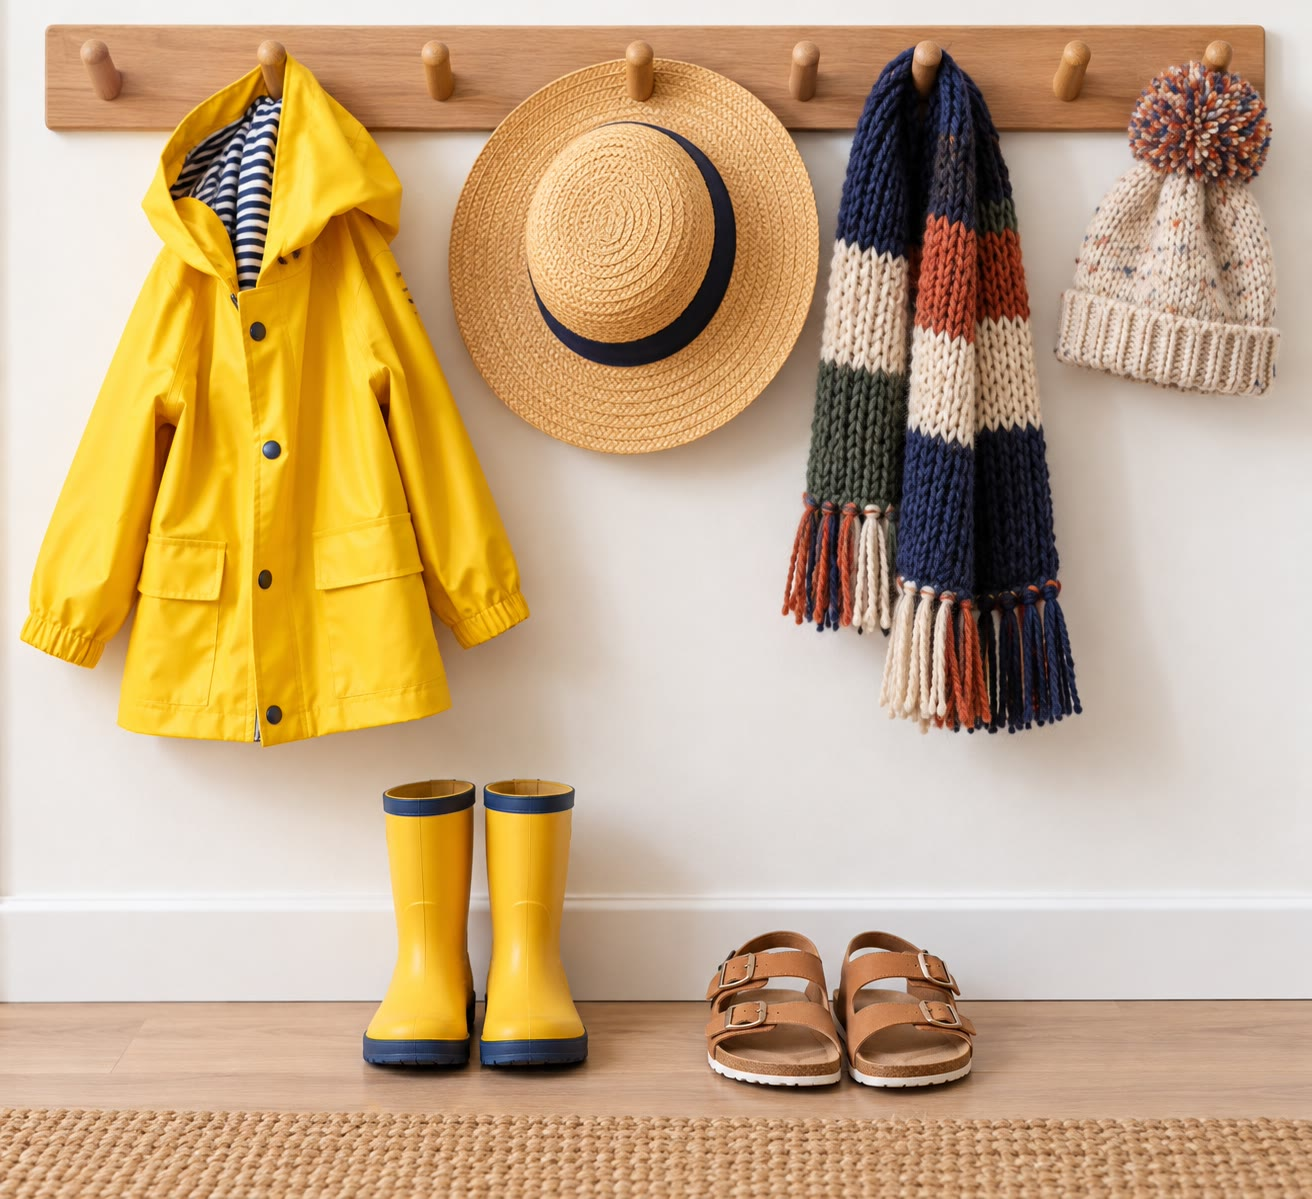
\includegraphics[width=0.66\linewidth]{images/book1/ai/g1-coat-pegs.jpg}

{\small Roupas para todo tipo de \omterm{def:g1:watching-the-weather:weather}{tempo}: uma capa de chuva, um chapéu de
sol, um cachecol e uma touca, botas e sandálias.}
\end{omfigure}

\begin{method}[Escolher a roupa de acordo com o tempo]\label{met:g1:watching-the-weather:clothes}
Olhe o céu e sinta o ar; depois:
\begin{itemize}
  \item chuva ou pancadas de chuva: capa de chuva ou guarda-chuva, e
        botas;
  \item frio ou neve: um casaco quente, cachecol, touca e luvas;
  \item sol forte e calor: chapéu de sol, roupa leve e água para beber;
  \item vento: um casaco que feche bem; o guarda-chuva não ajuda muito.
\end{itemize}
\end{method}

\begin{safety}
\textbf{Nunca olhe diretamente para o Sol}, nem por um instante, e nunca
através de óculos, binóculos ou de uma câmera: isso pode machucar os seus
olhos para sempre. Quando houver uma trovoada, fique dentro de casa ou de
um carro, longe de árvores altas e da água, e espere a tempestade passar.
\end{safety}

\section{Exercícios}

\begin{exercise}[$\star$]\label{exo:g1:watching-the-weather:1}
Desenhe o símbolo de cada tipo de \omterm{def:g1:watching-the-weather:weather}{tempo}: ensolarado; chuvoso; com neve; nublado.
\end{exercise}

\begin{exercise}[$\star$]\label{exo:g1:watching-the-weather:2}
Como está o \omterm{def:g1:watching-the-weather:weather}{tempo} em cada uma das quatro fotos da seção ``O que é o
\omterm{def:g1:watching-the-weather:weather}{tempo}?''? Use uma ou duas palavras para cada uma.
\end{exercise}

\begin{exercise}[$\star$]\label{exo:g1:watching-the-weather:3}
Observe o \omterm{def:g1:watching-the-weather:weather-chart}{quadro do tempo} da turma. Como estava o \omterm{def:g1:watching-the-weather:weather}{tempo} na manhã de
terça-feira? Na tarde de sexta-feira? Na tarde de domingo?
\end{exercise}

\begin{exercise}[$\star$]\label{exo:g1:watching-the-weather:4}
No \omterm{def:g1:watching-the-weather:weather-chart}{quadro do tempo} da turma, em que dia fez sol de manhã e também à
tarde?
\end{exercise}

\begin{exercise}[$\star$]\label{exo:g1:watching-the-weather:5}
Ligue cada peça de roupa a um tipo de \omterm{def:g1:watching-the-weather:weather}{tempo}: um chapéu de sol; botas e
uma capa de chuva; um cachecol e luvas. Os tipos de \omterm{def:g1:watching-the-weather:weather}{tempo} são: frio e
com neve; quente e ensolarado; chuvoso.
\end{exercise}

\begin{exercise}[$\star$]\label{exo:g1:watching-the-weather:6}
Lena diz: ``Olhe, a bandeira está tremulando!'' Como está o \omterm{def:g1:watching-the-weather:weather}{tempo}?
\end{exercise}

\begin{exercise}[$\star$]\label{exo:g1:watching-the-weather:7}
Verdadeiro ou falso? Explique.
\begin{enumerate}
  \item O \omterm{def:g1:watching-the-weather:weather}{tempo} é sempre igual de manhã e à tarde.
  \item A neblina é uma nuvem que encosta no chão.
  \item A regra ``nunca olhe para o Sol, nem com um olho só'' é uma boa regra.
\end{enumerate}
\end{exercise}

\begin{exercise}[$\star\star$]\label{exo:g1:watching-the-weather:8}
No \omterm{def:g1:watching-the-weather:weather-chart}{quadro do tempo} da turma, conte as tardes com chuva ou pancadas de
chuva. Conte os dias frios. A semana foi mais quente ou mais fria?
\end{exercise}

\begin{exercise}[$\star\star$]\label{exo:g1:watching-the-weather:9}
Veja o que Sam viu da janela durante um dia: de manhã, um céu cinzento;
na hora do almoço, gotas na janela; à noite, um céu azul com algumas
nuvens. Desenhe os três \omterm{def:g1:watching-the-weather:weather-chart}{símbolos do tempo} na ordem certa.
\end{exercise}

\begin{exercise}[$\star\star$]\label{exo:g1:watching-the-weather:10}
No desenho da biruta e da bandeira, o vento vem da esquerda. Num outro
dia, uma bandeira aponta para a esquerda. De que lado vem o vento nesse
dia?
\end{exercise}

\begin{exercise}[$\star\star$]\label{exo:g1:watching-the-weather:11}
Observe o desenho da mesma árvore nas quatro estações. Em que estação a
árvore está sem folhas? Em que estação ela tem flores? Que \omterm{def:g1:watching-the-weather:weather-chart}{símbolo do
tempo} foi desenhado no inverno, e por que ele combina com essa estação?
\end{exercise}
